% !TEX encoding = UTF-8 Unicode

\documentclass{standalone}
%\documentclass{article}

% packages
\usepackage{float}
\usepackage{tabu}
\usepackage{booktabs}
\usepackage{graphicx}
\usepackage{caption}
\usepackage[export]{adjustbox}
\usepackage[utf8]{inputenc}
%\usepackage[active,pdftex,tightpage]{preview}

\begin{document}


%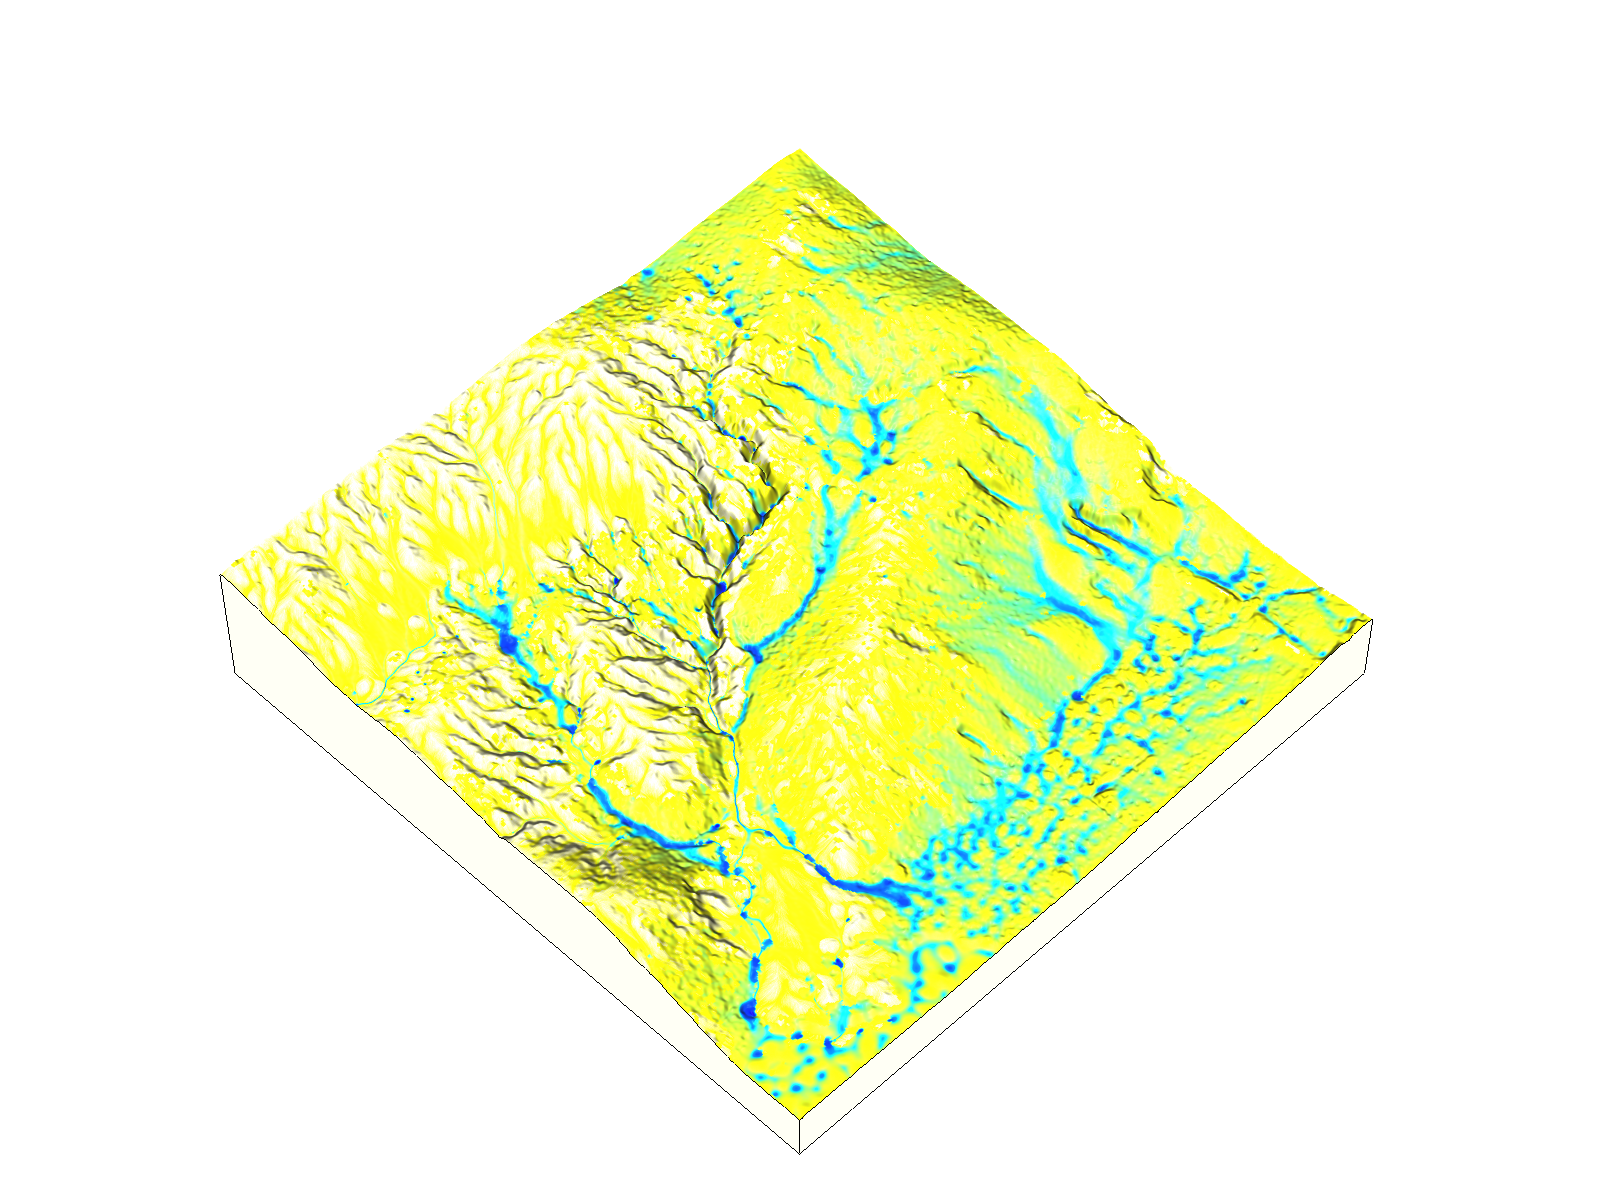
\includegraphics[width=0.5\textwidth]{../../images/sample_data_3d/depth_2016.png}


%\begin{figure}[h]
\small\sf\centering
\begin{tabular}{m{0.5\textwidth} m{0.5\textwidth}}
%
%\multicolumn{1}{c}{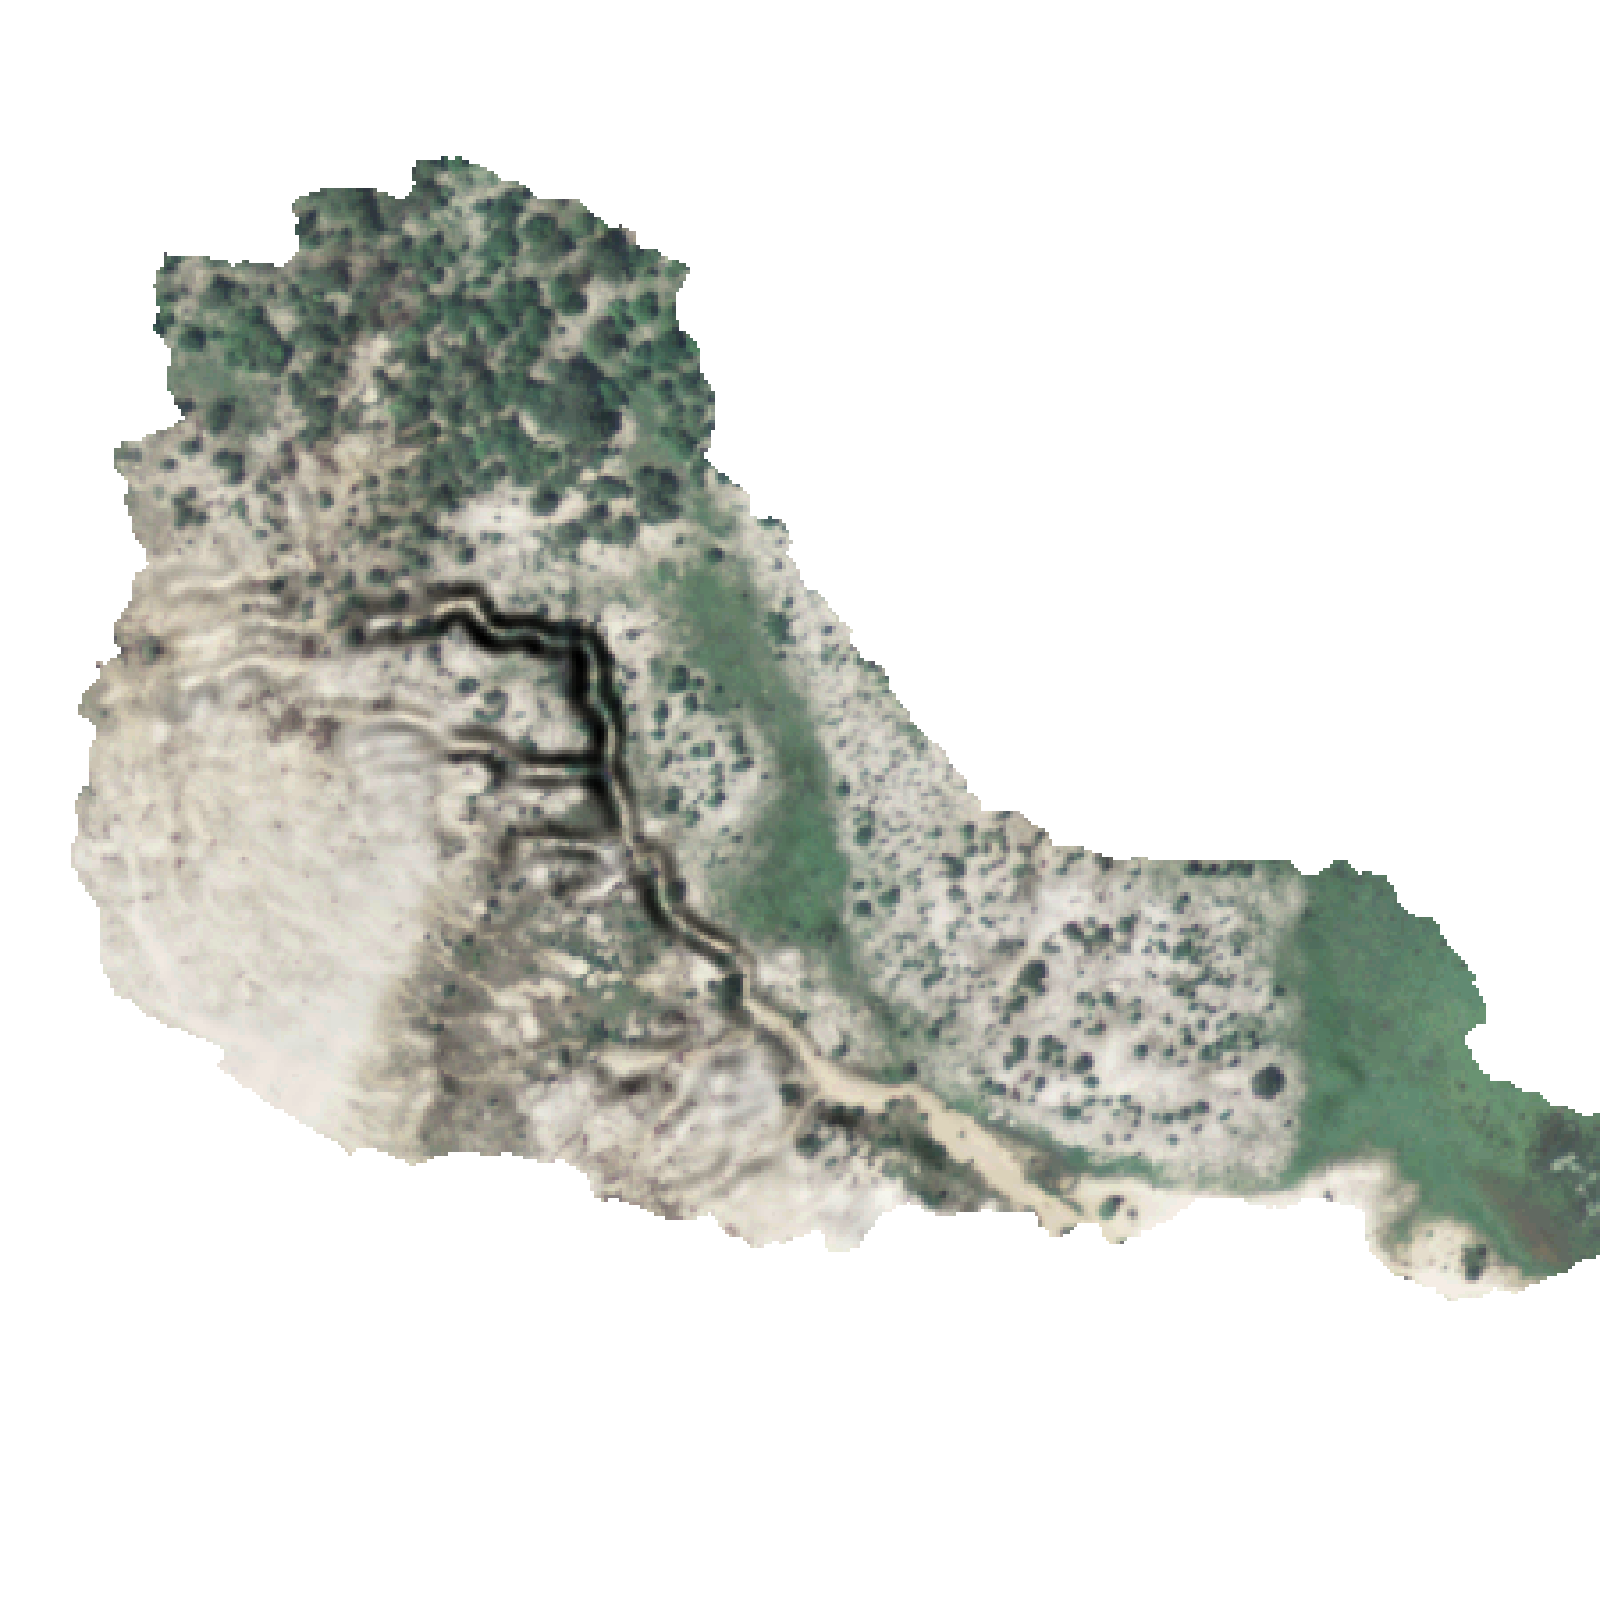
\includegraphics[height=60mm]{../../images/sample_data/naip_2014.png}} &
%\multicolumn{1}{c}{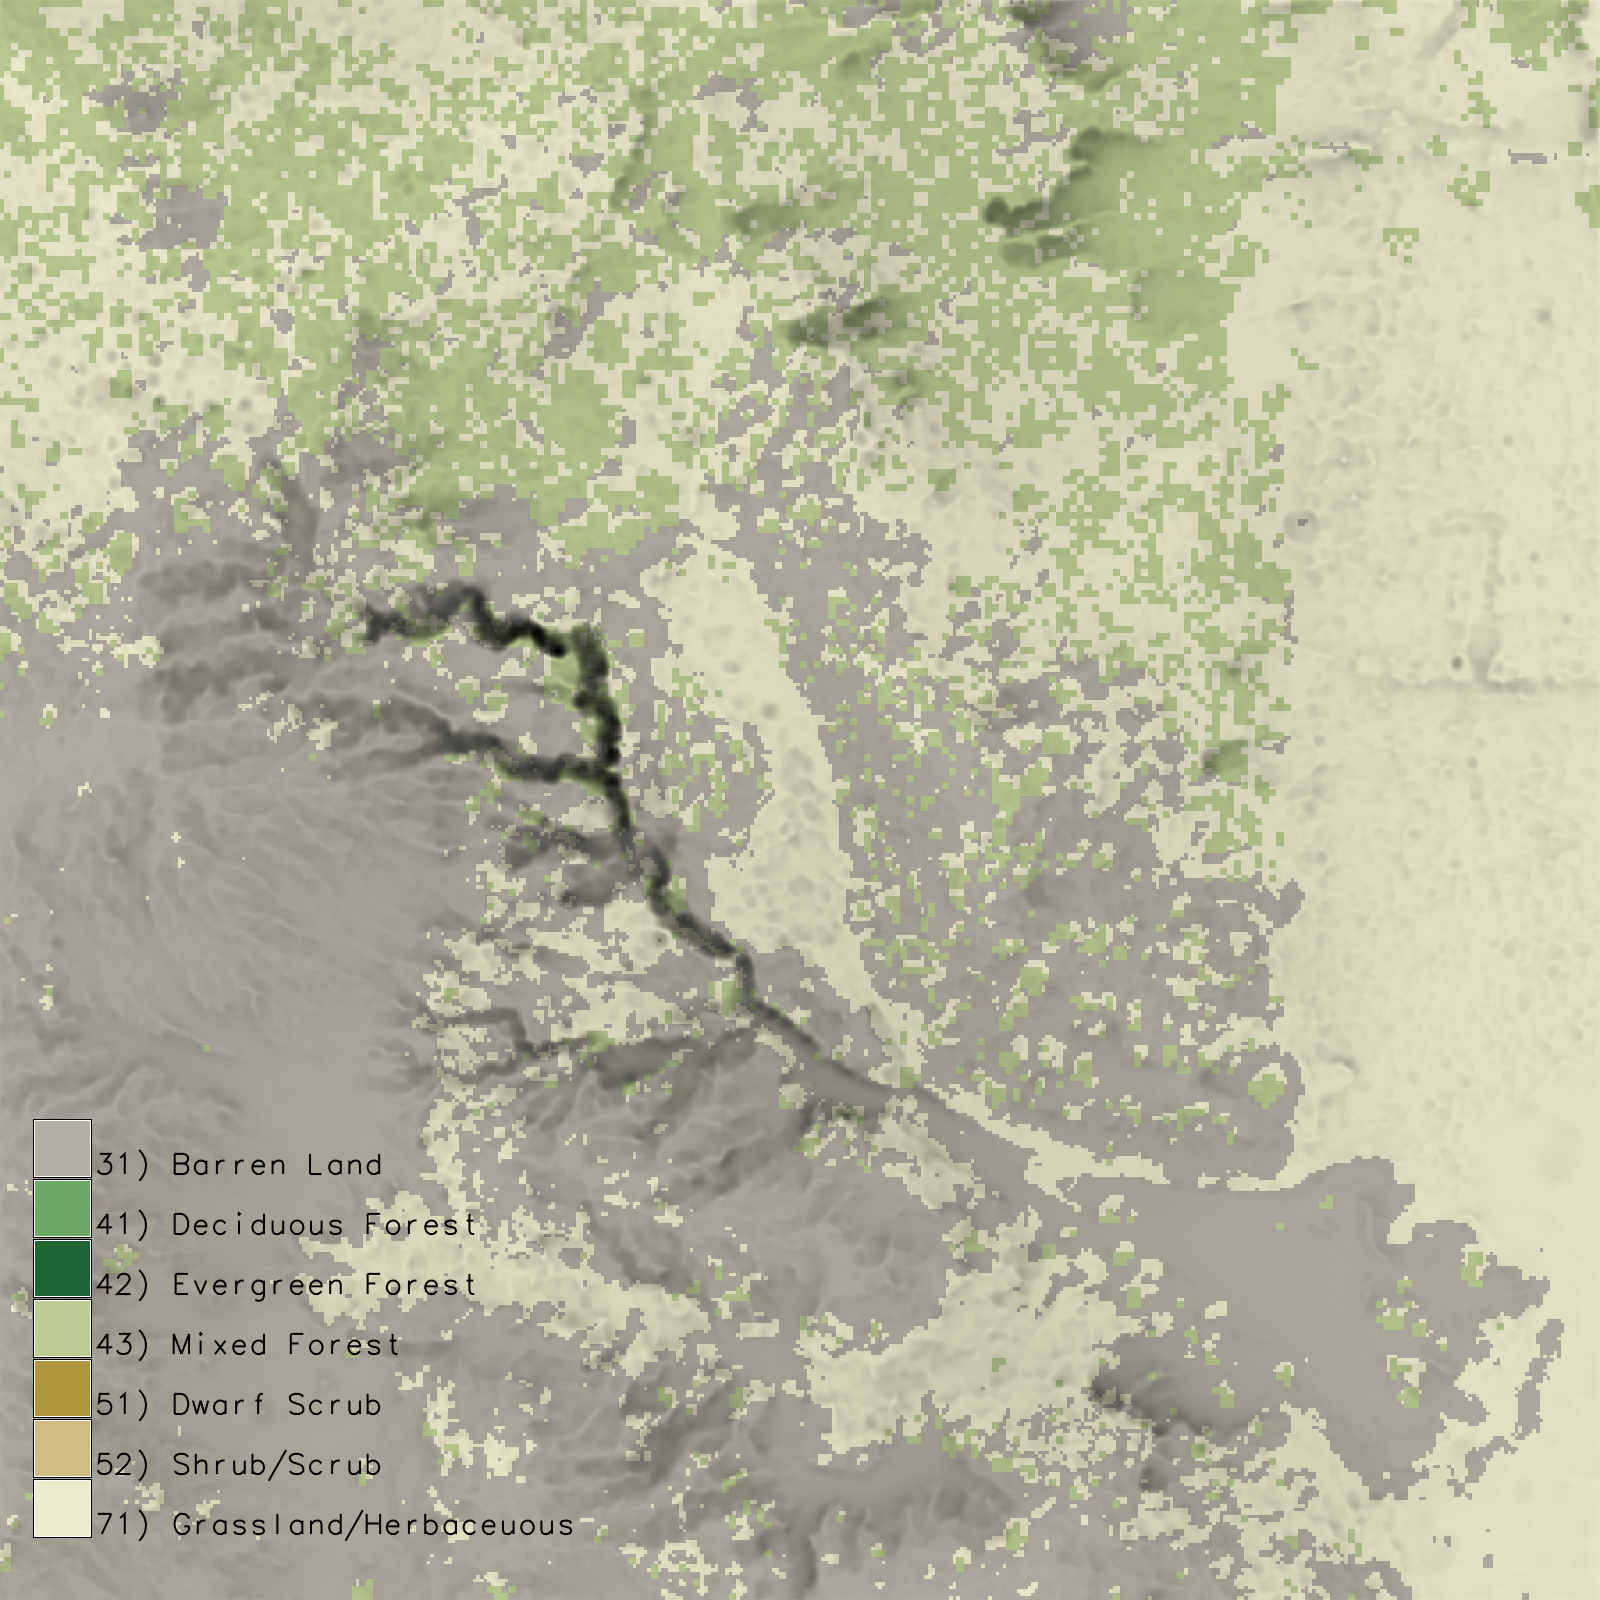
\includegraphics[height=60mm]{../../images/sample_data/landcover.png}}\\
%\multicolumn{1}{c}{a. Orthophotograph} & \multicolumn{1}{c}{b. Landcover}\\
%
\multicolumn{1}{c}{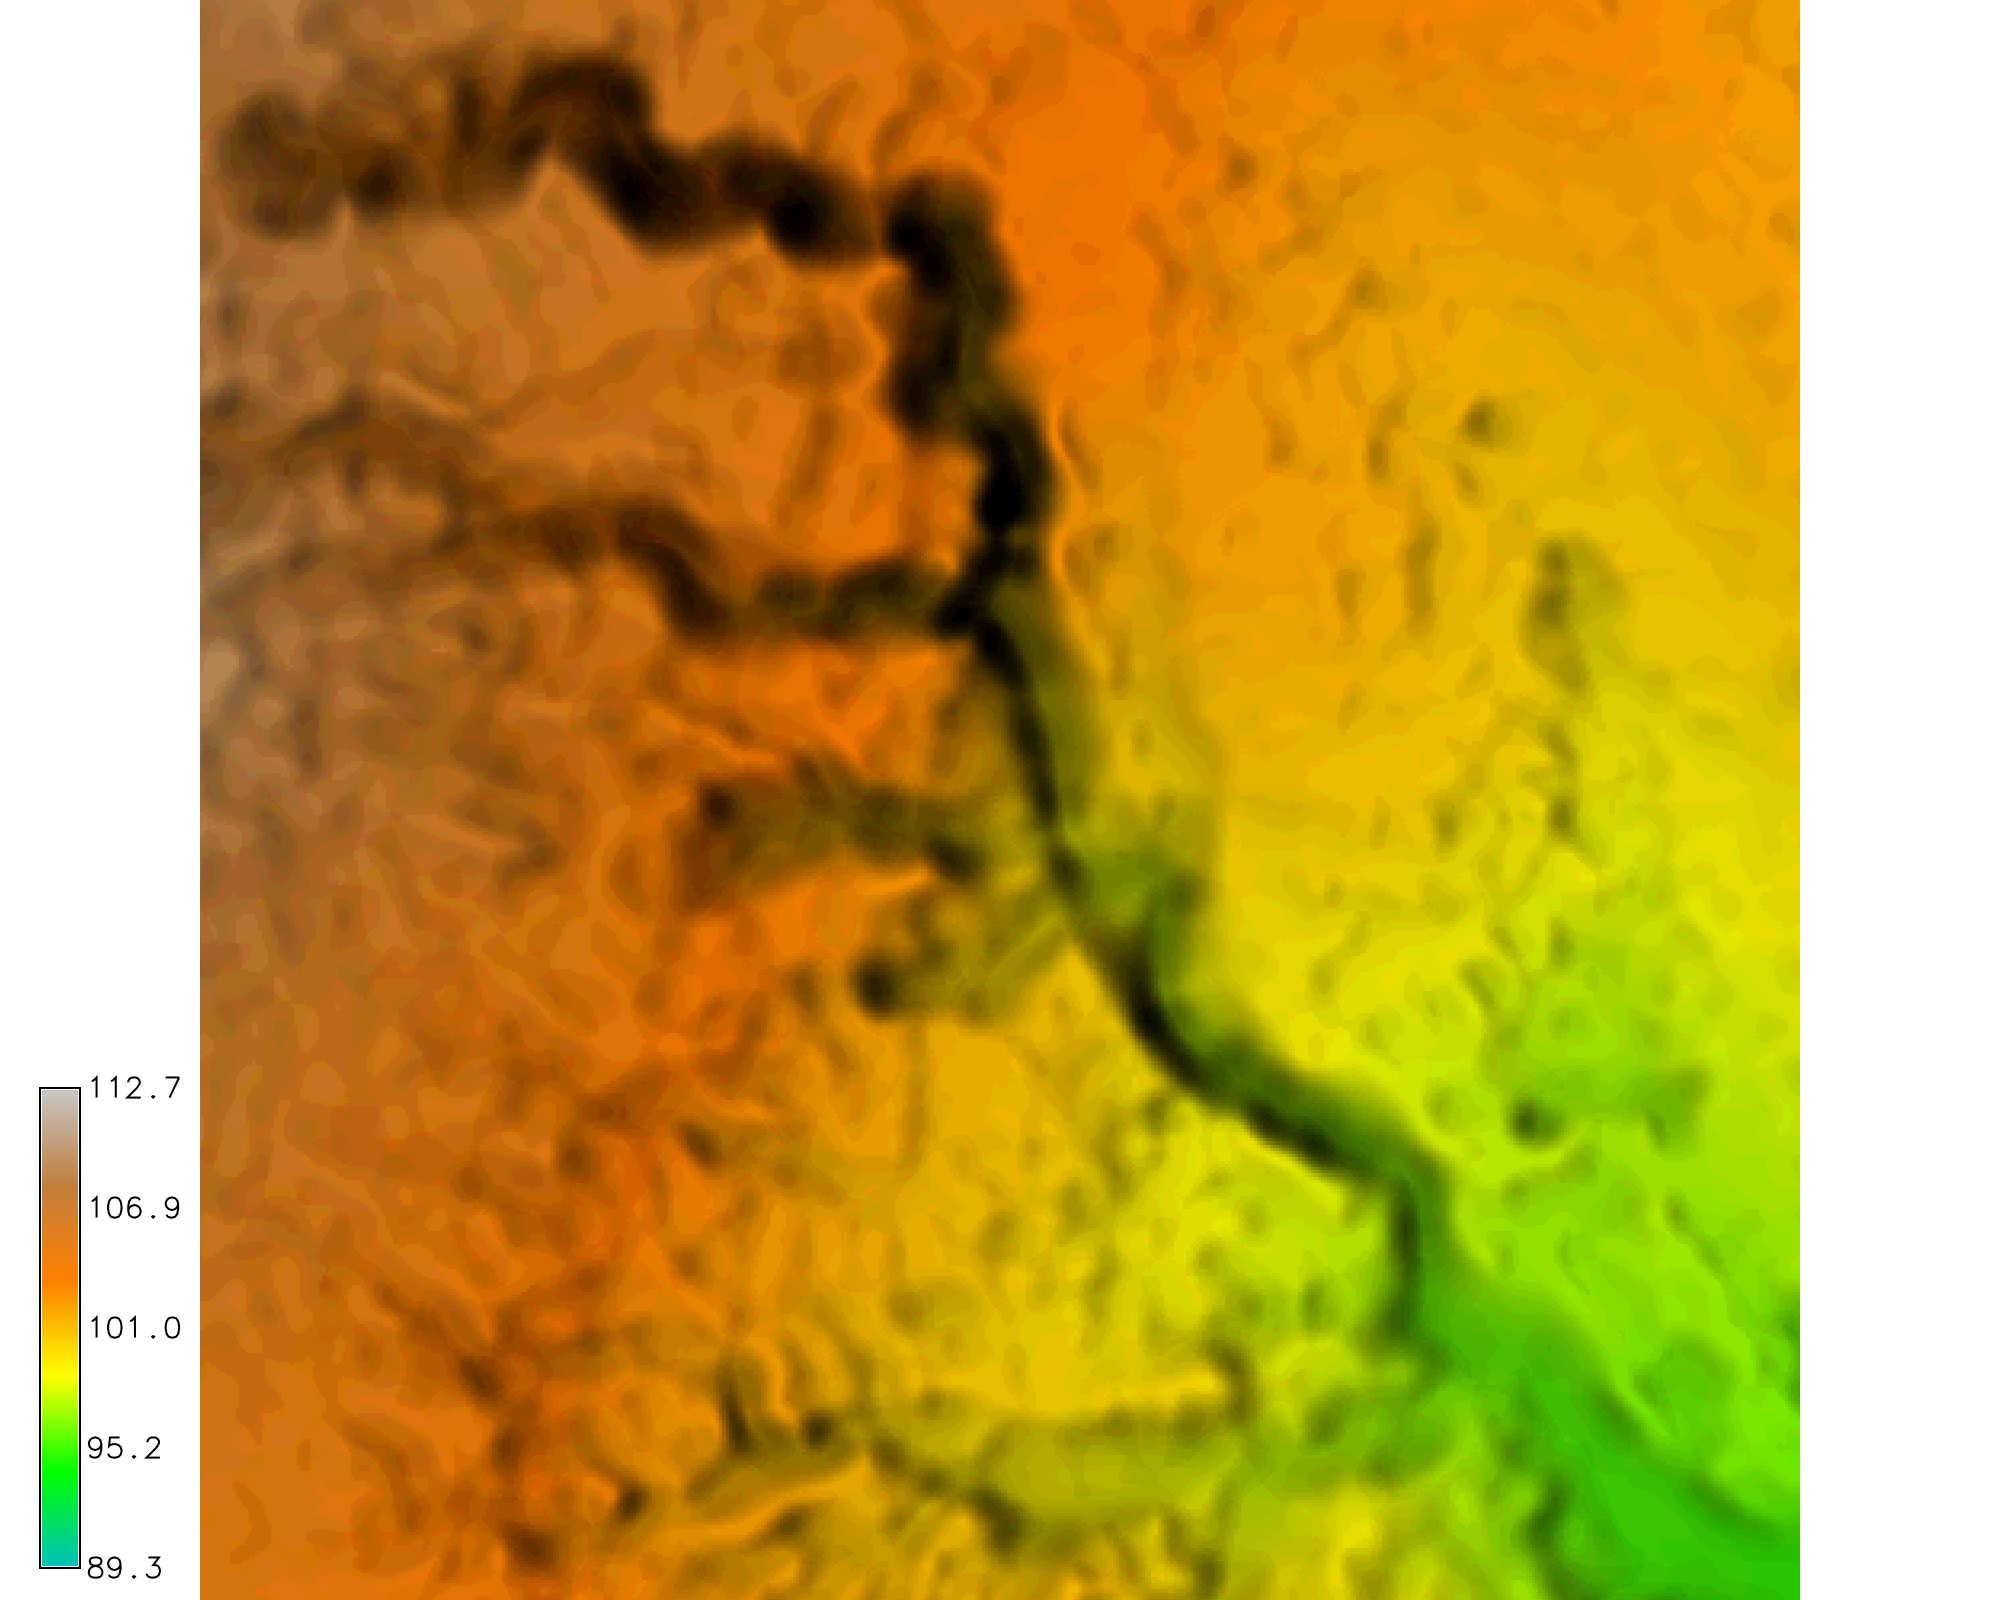
\includegraphics[height=60mm]{../../images/sample_data/gully_elevation_2012.png}} &
\multicolumn{1}{c}{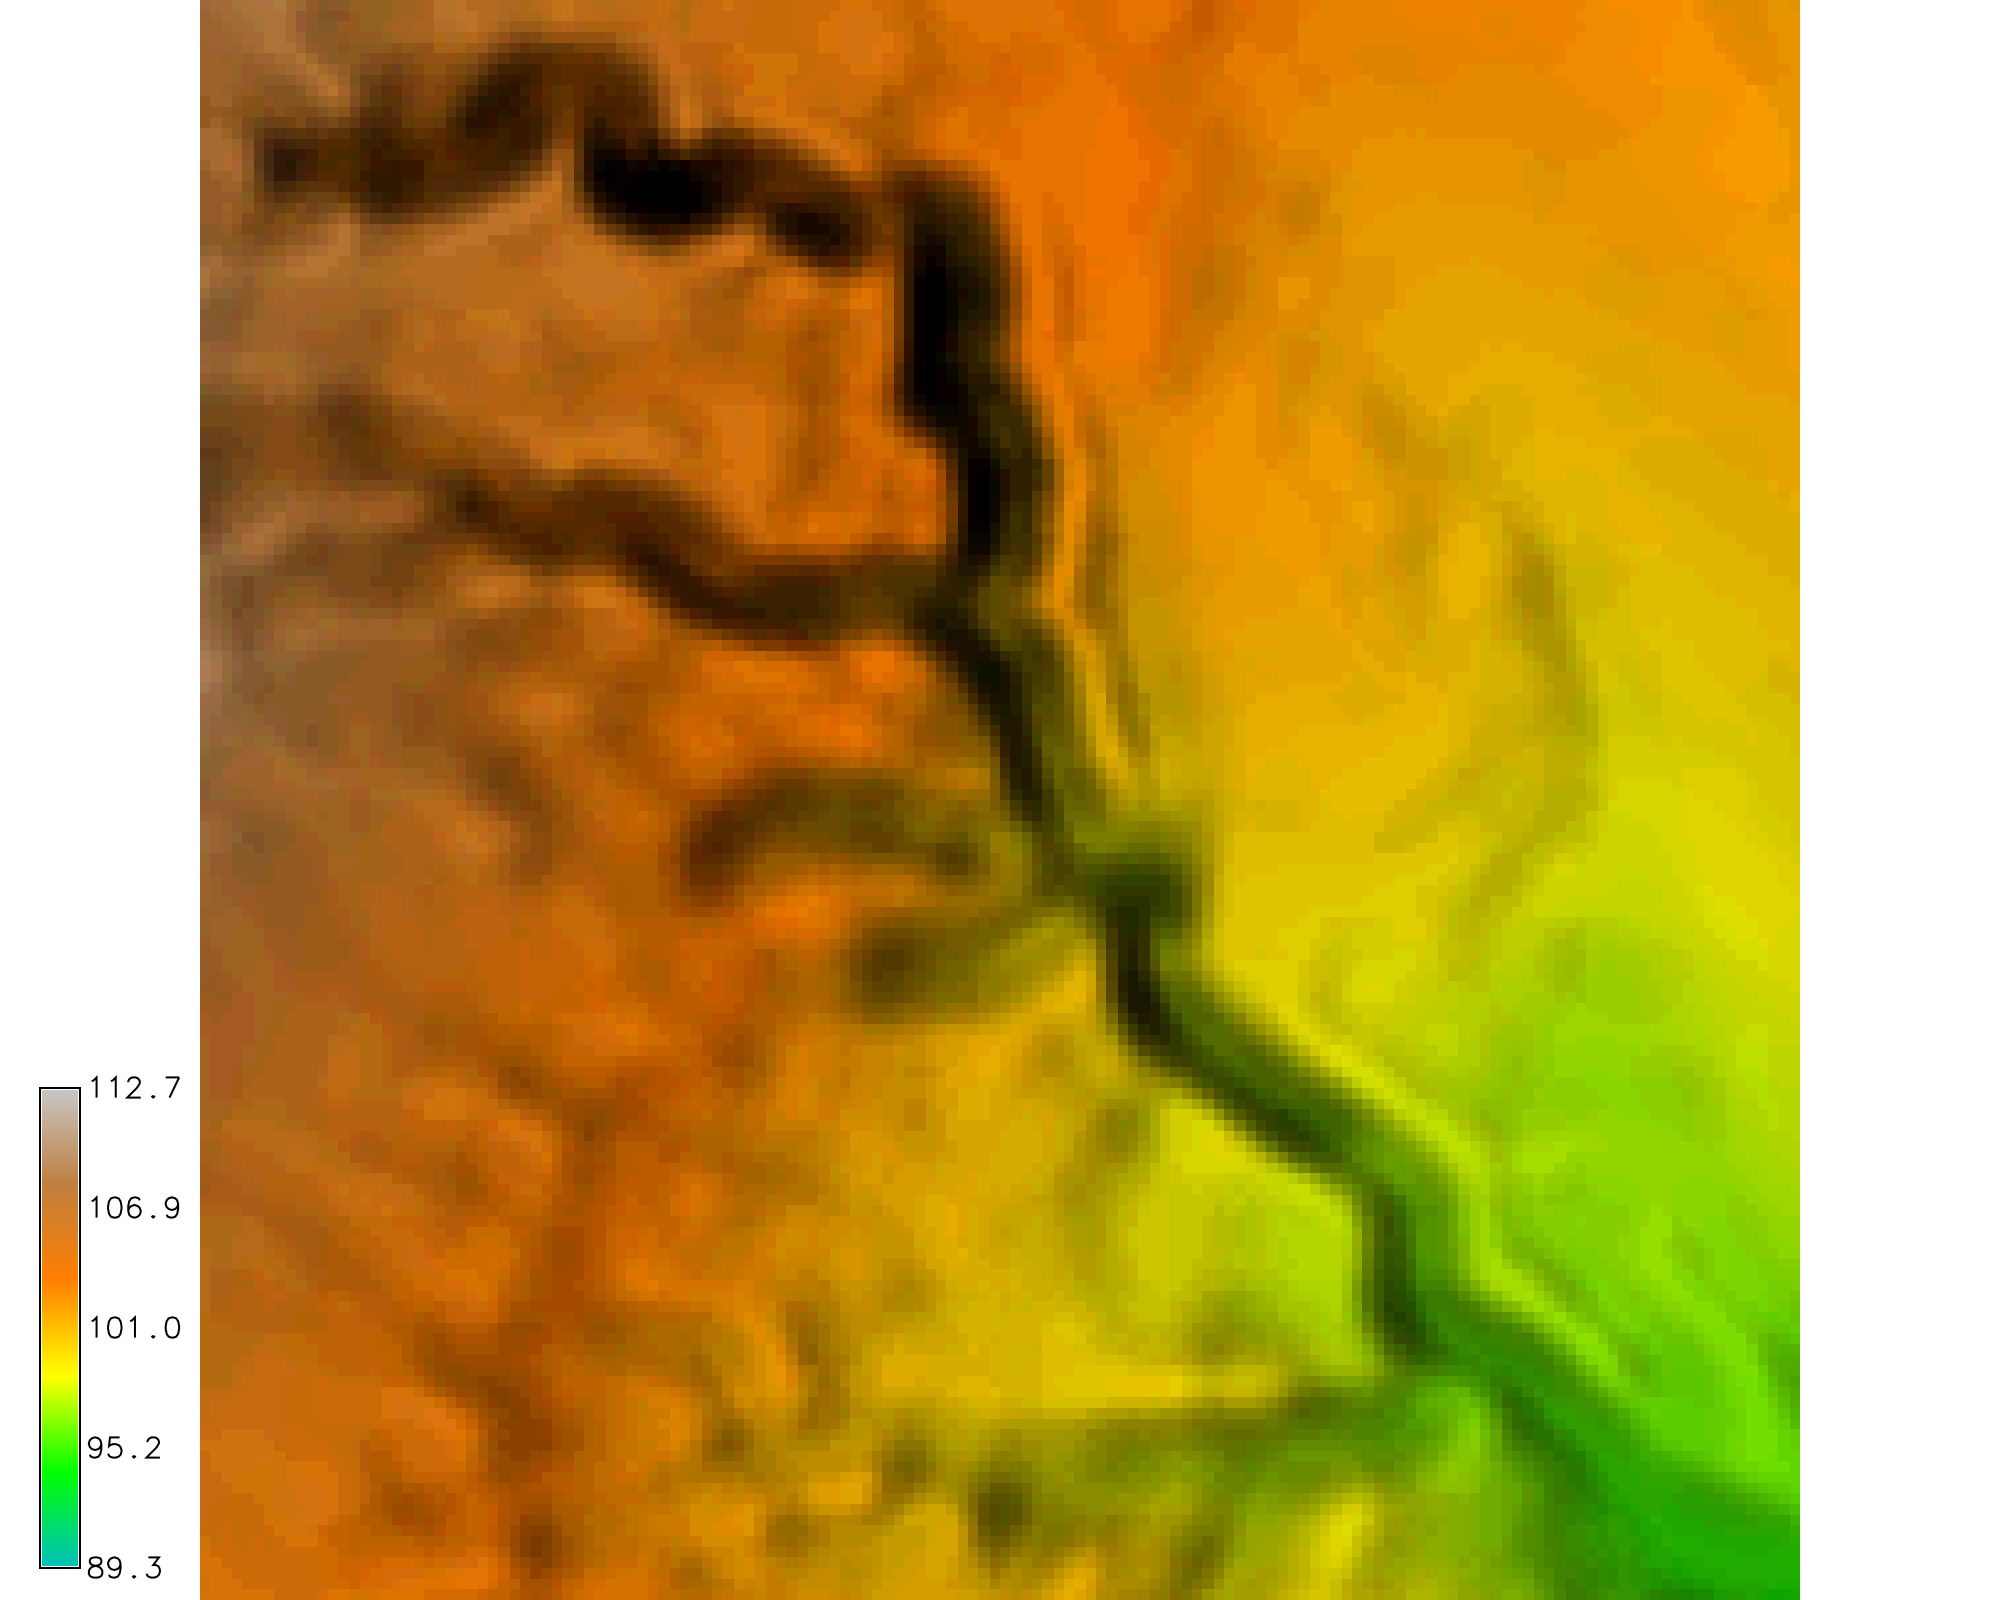
\includegraphics[height=60mm]{../../images/sample_data/gully_elevation_2016.png}}\\
\multicolumn{1}{c}{a. Elevation 2012} & \multicolumn{1}{c}{b. Elevation 2016}\\
%
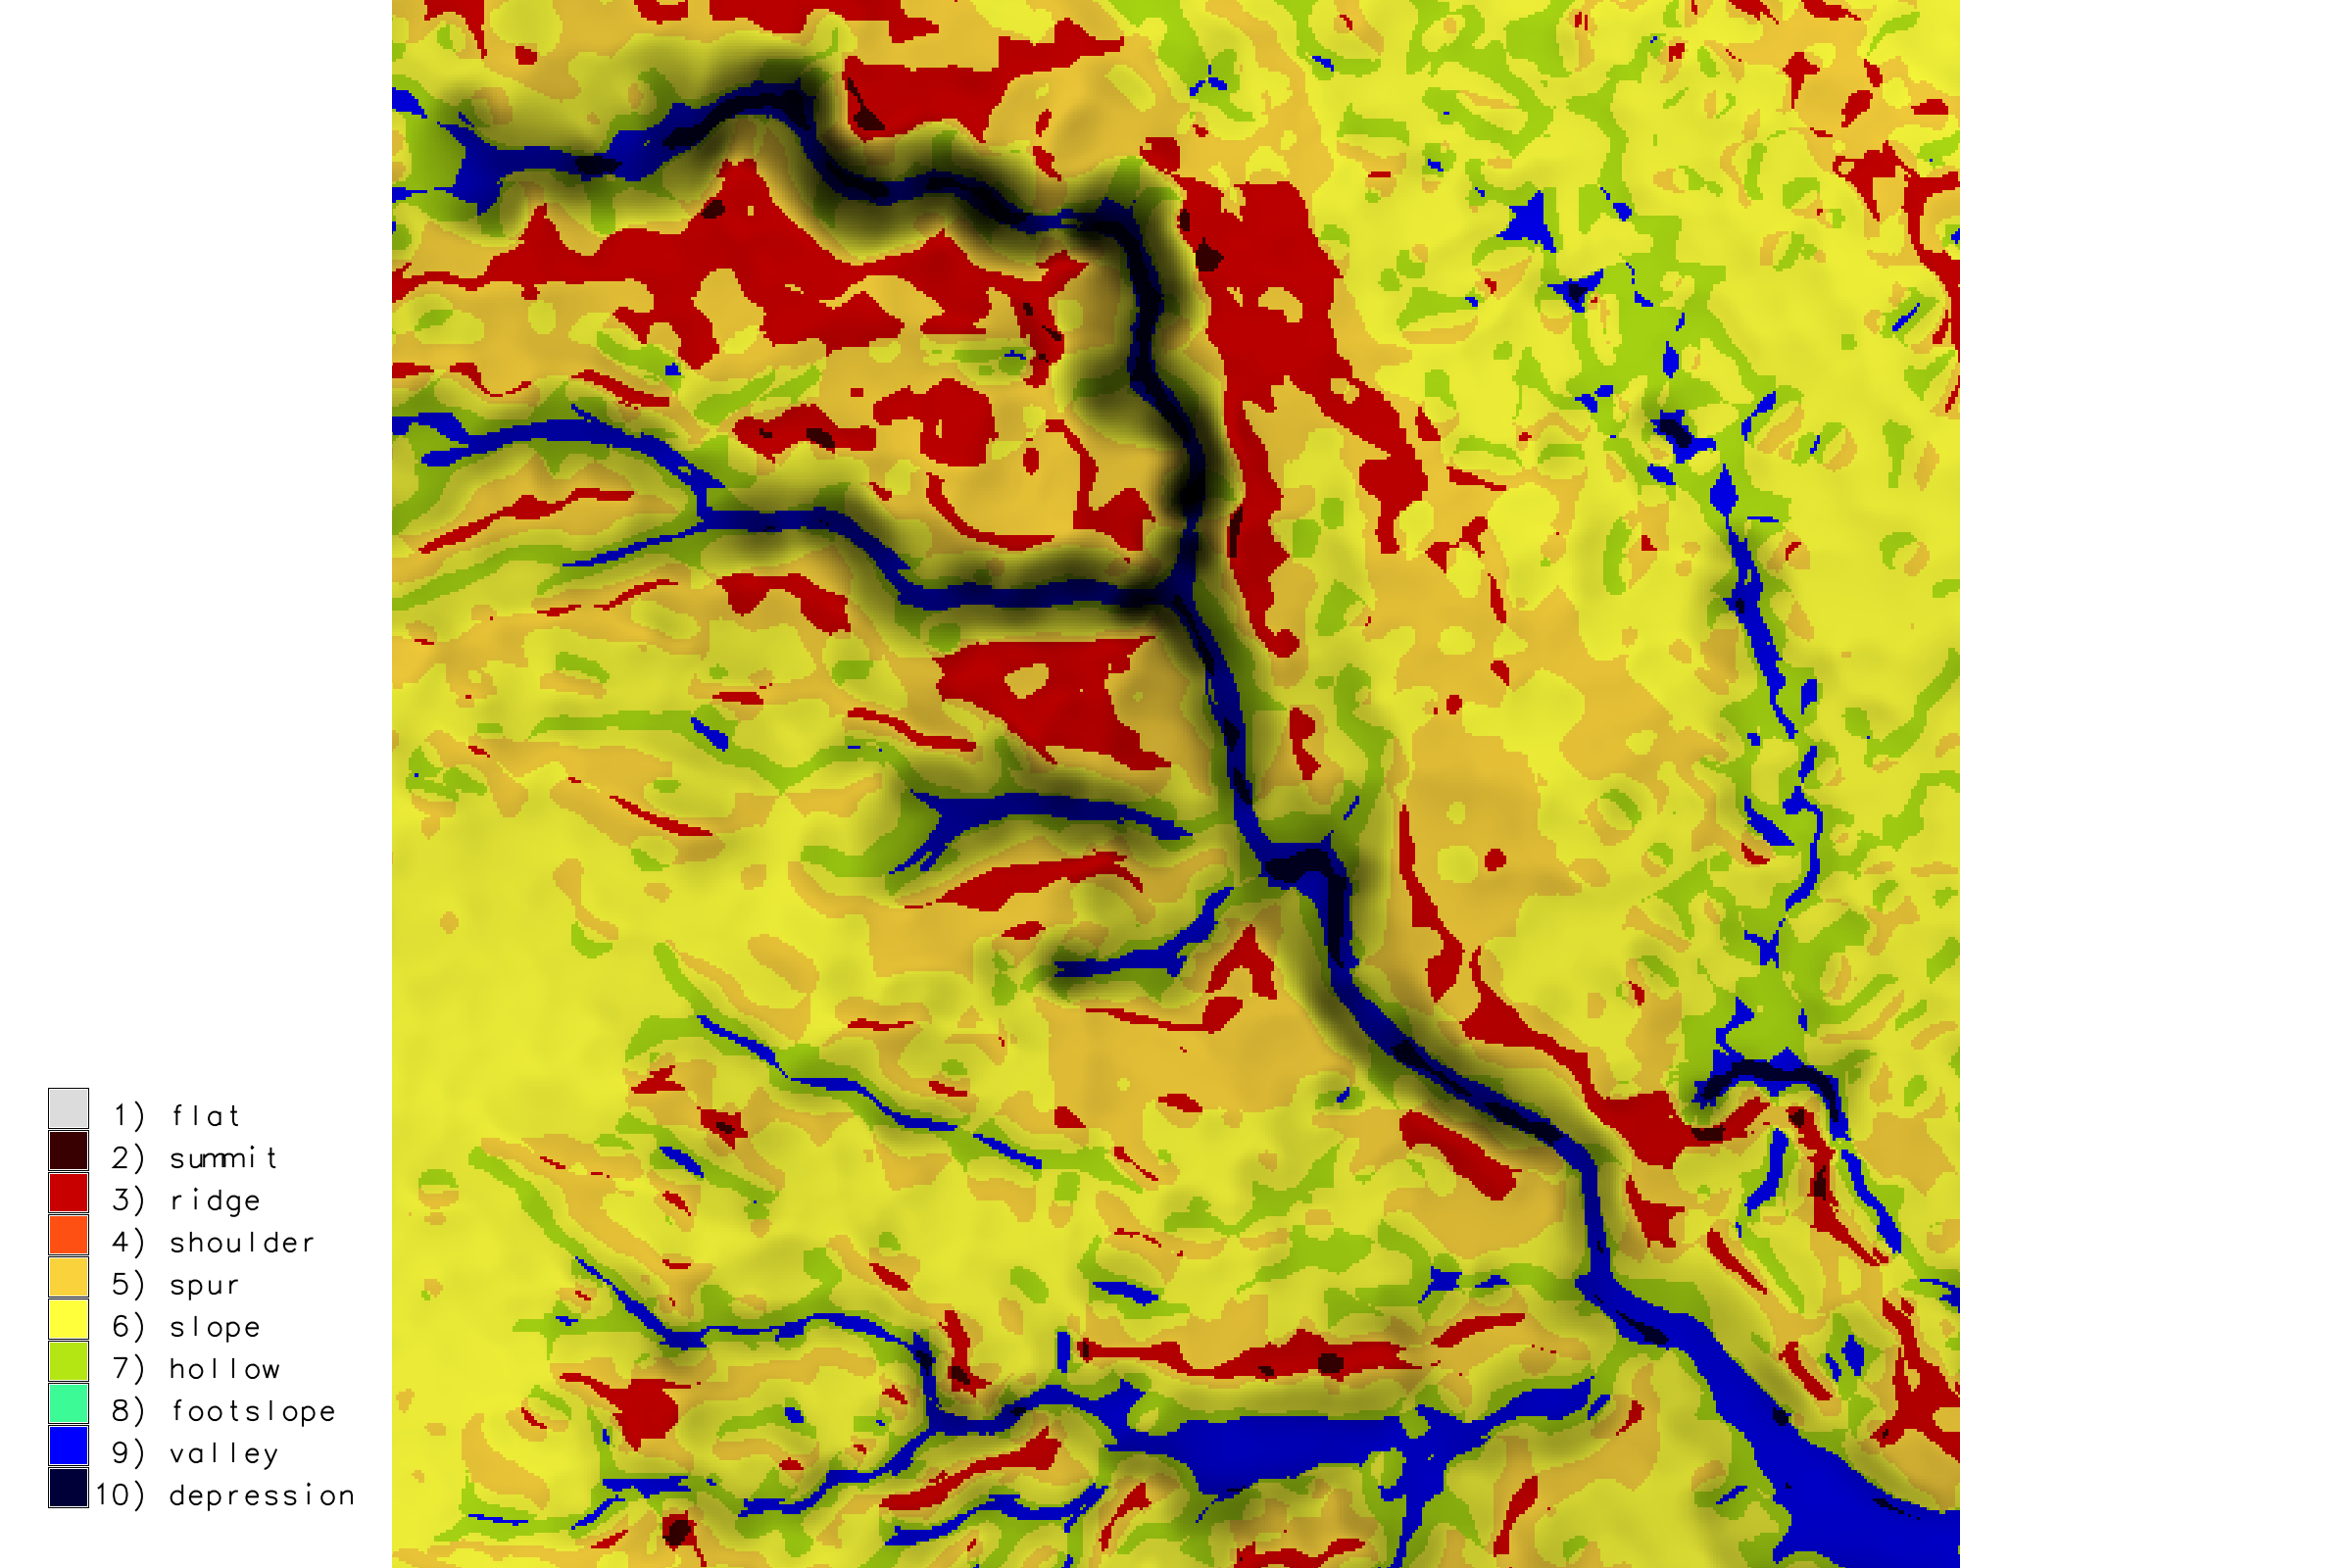
\includegraphics[height=60mm,center]{../../images/sample_data/gully_landforms_2012.png} &
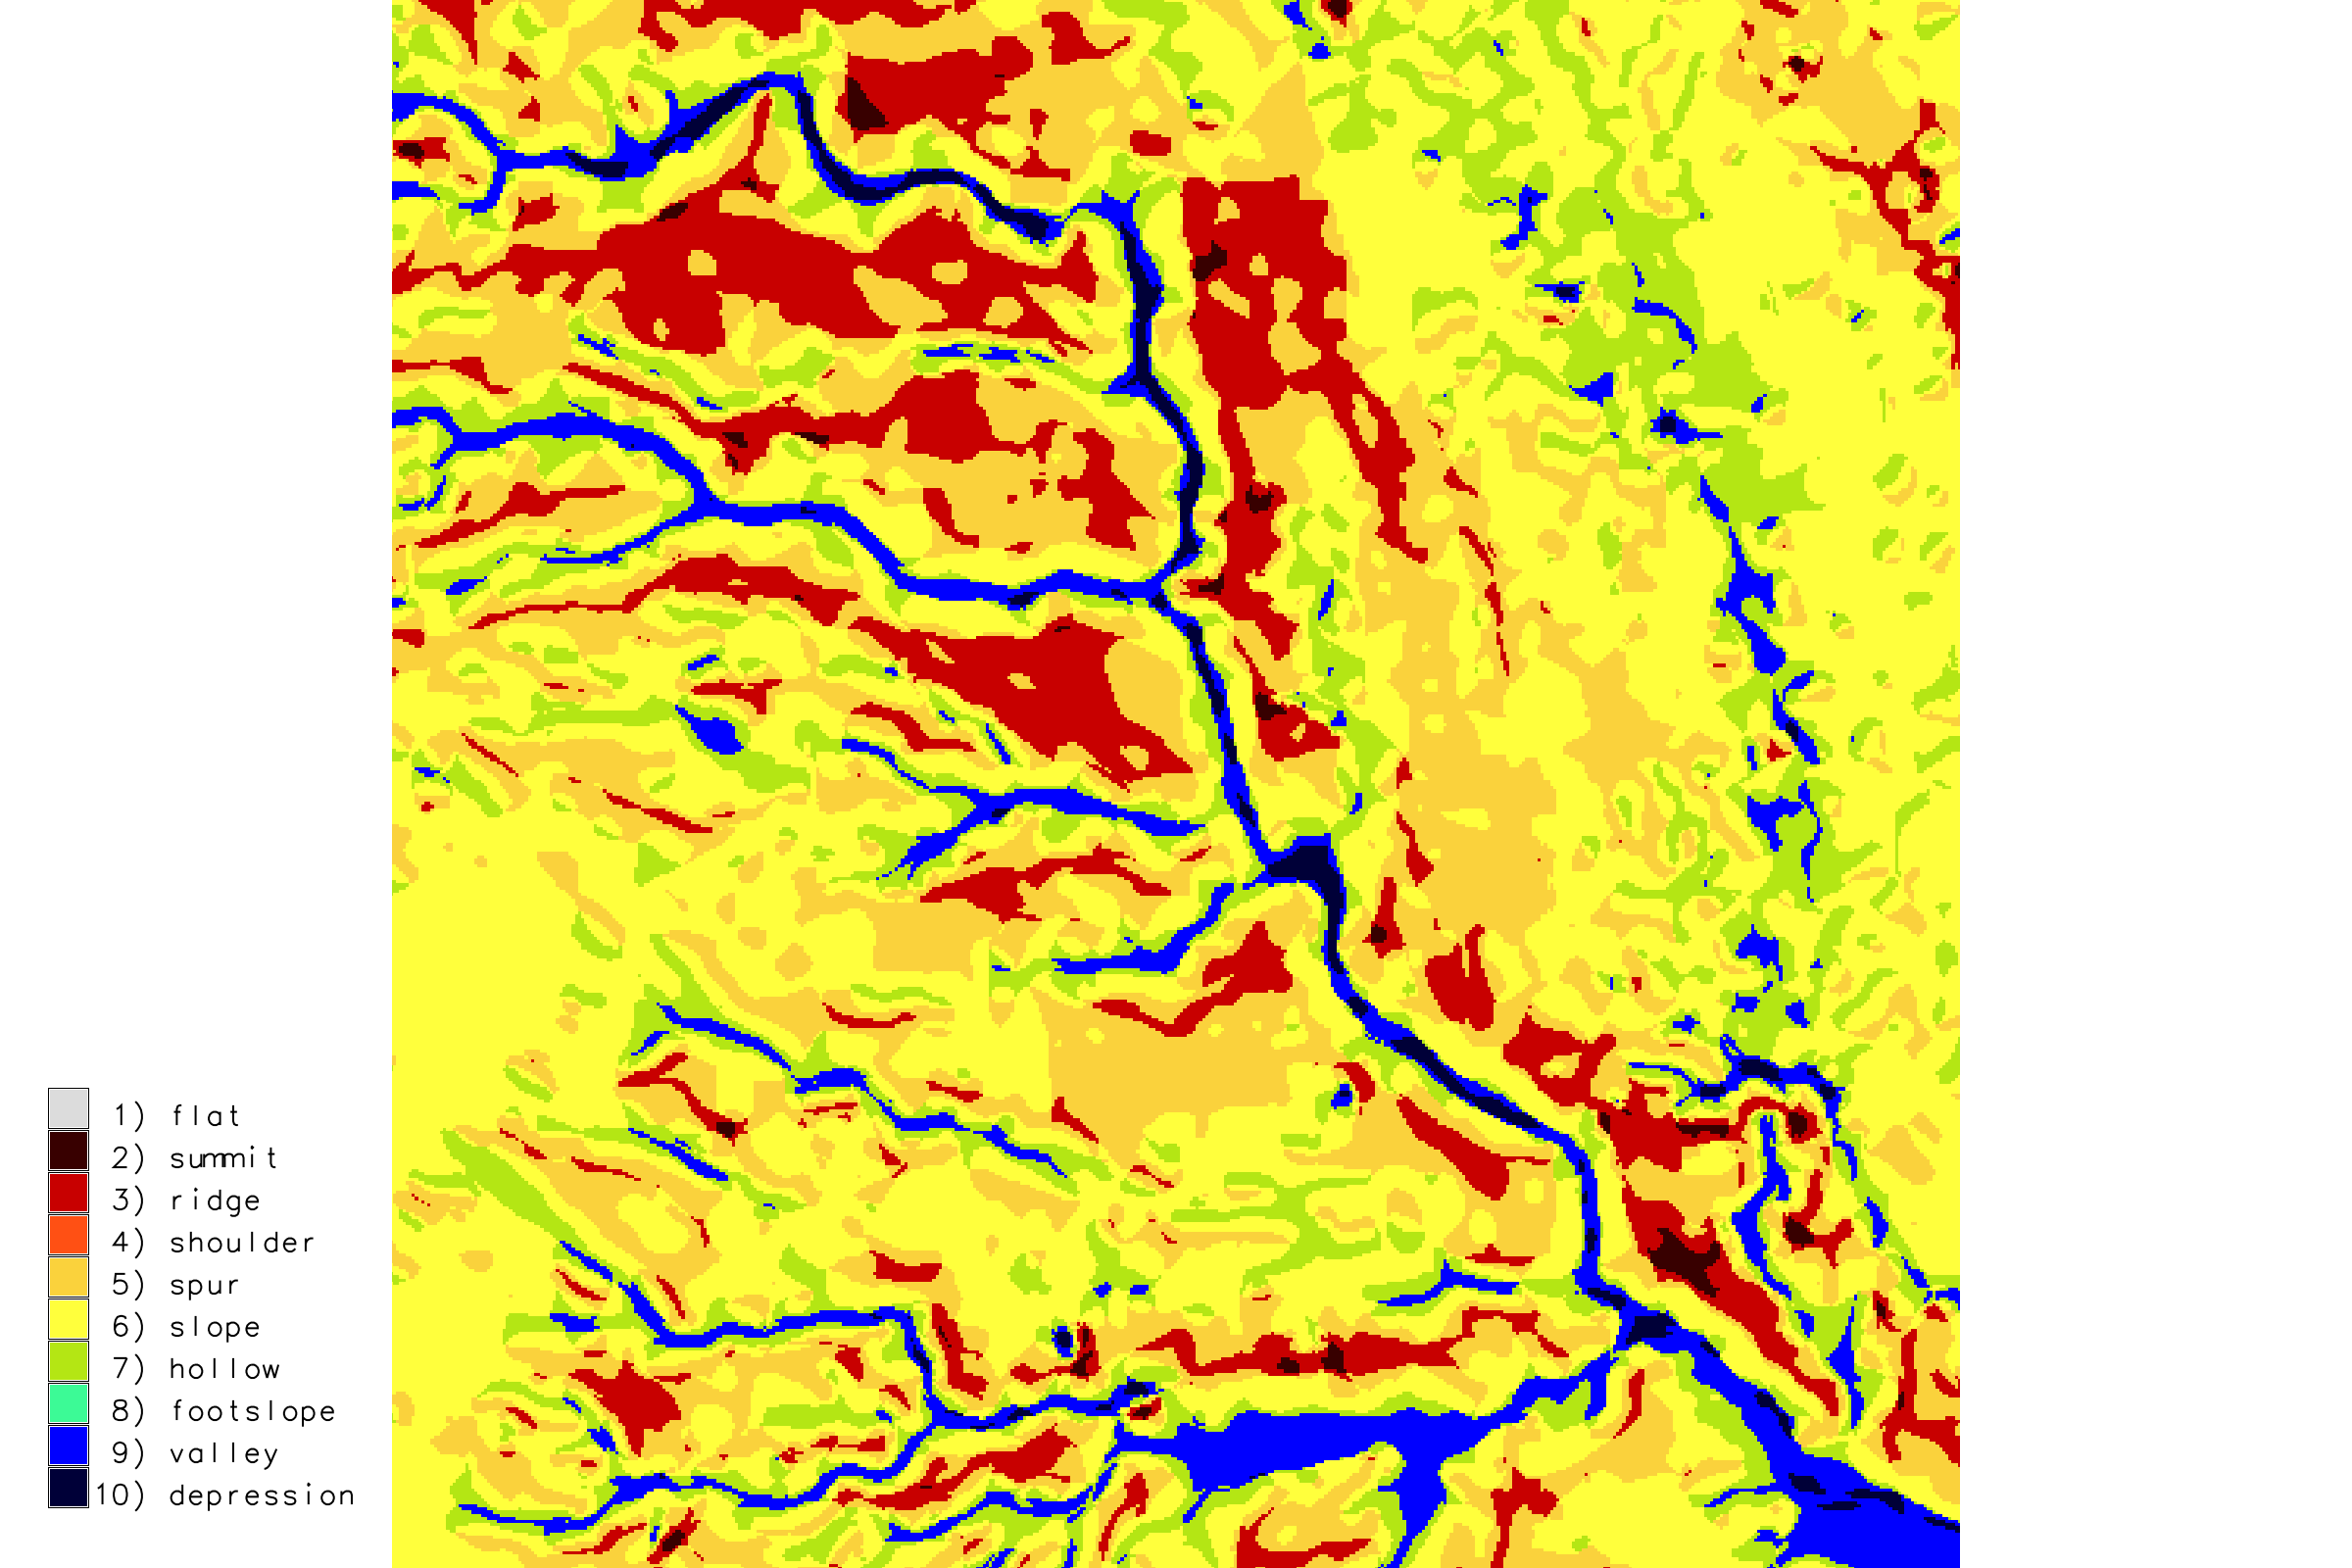
\includegraphics[height=60mm,center]{../../images/sample_data/gully_landforms_2016.png}\\
\multicolumn{1}{c}{c. Landforms 2012} & \multicolumn{1}{c}{d. Landforms 2016}\\
%
\multicolumn{1}{c}{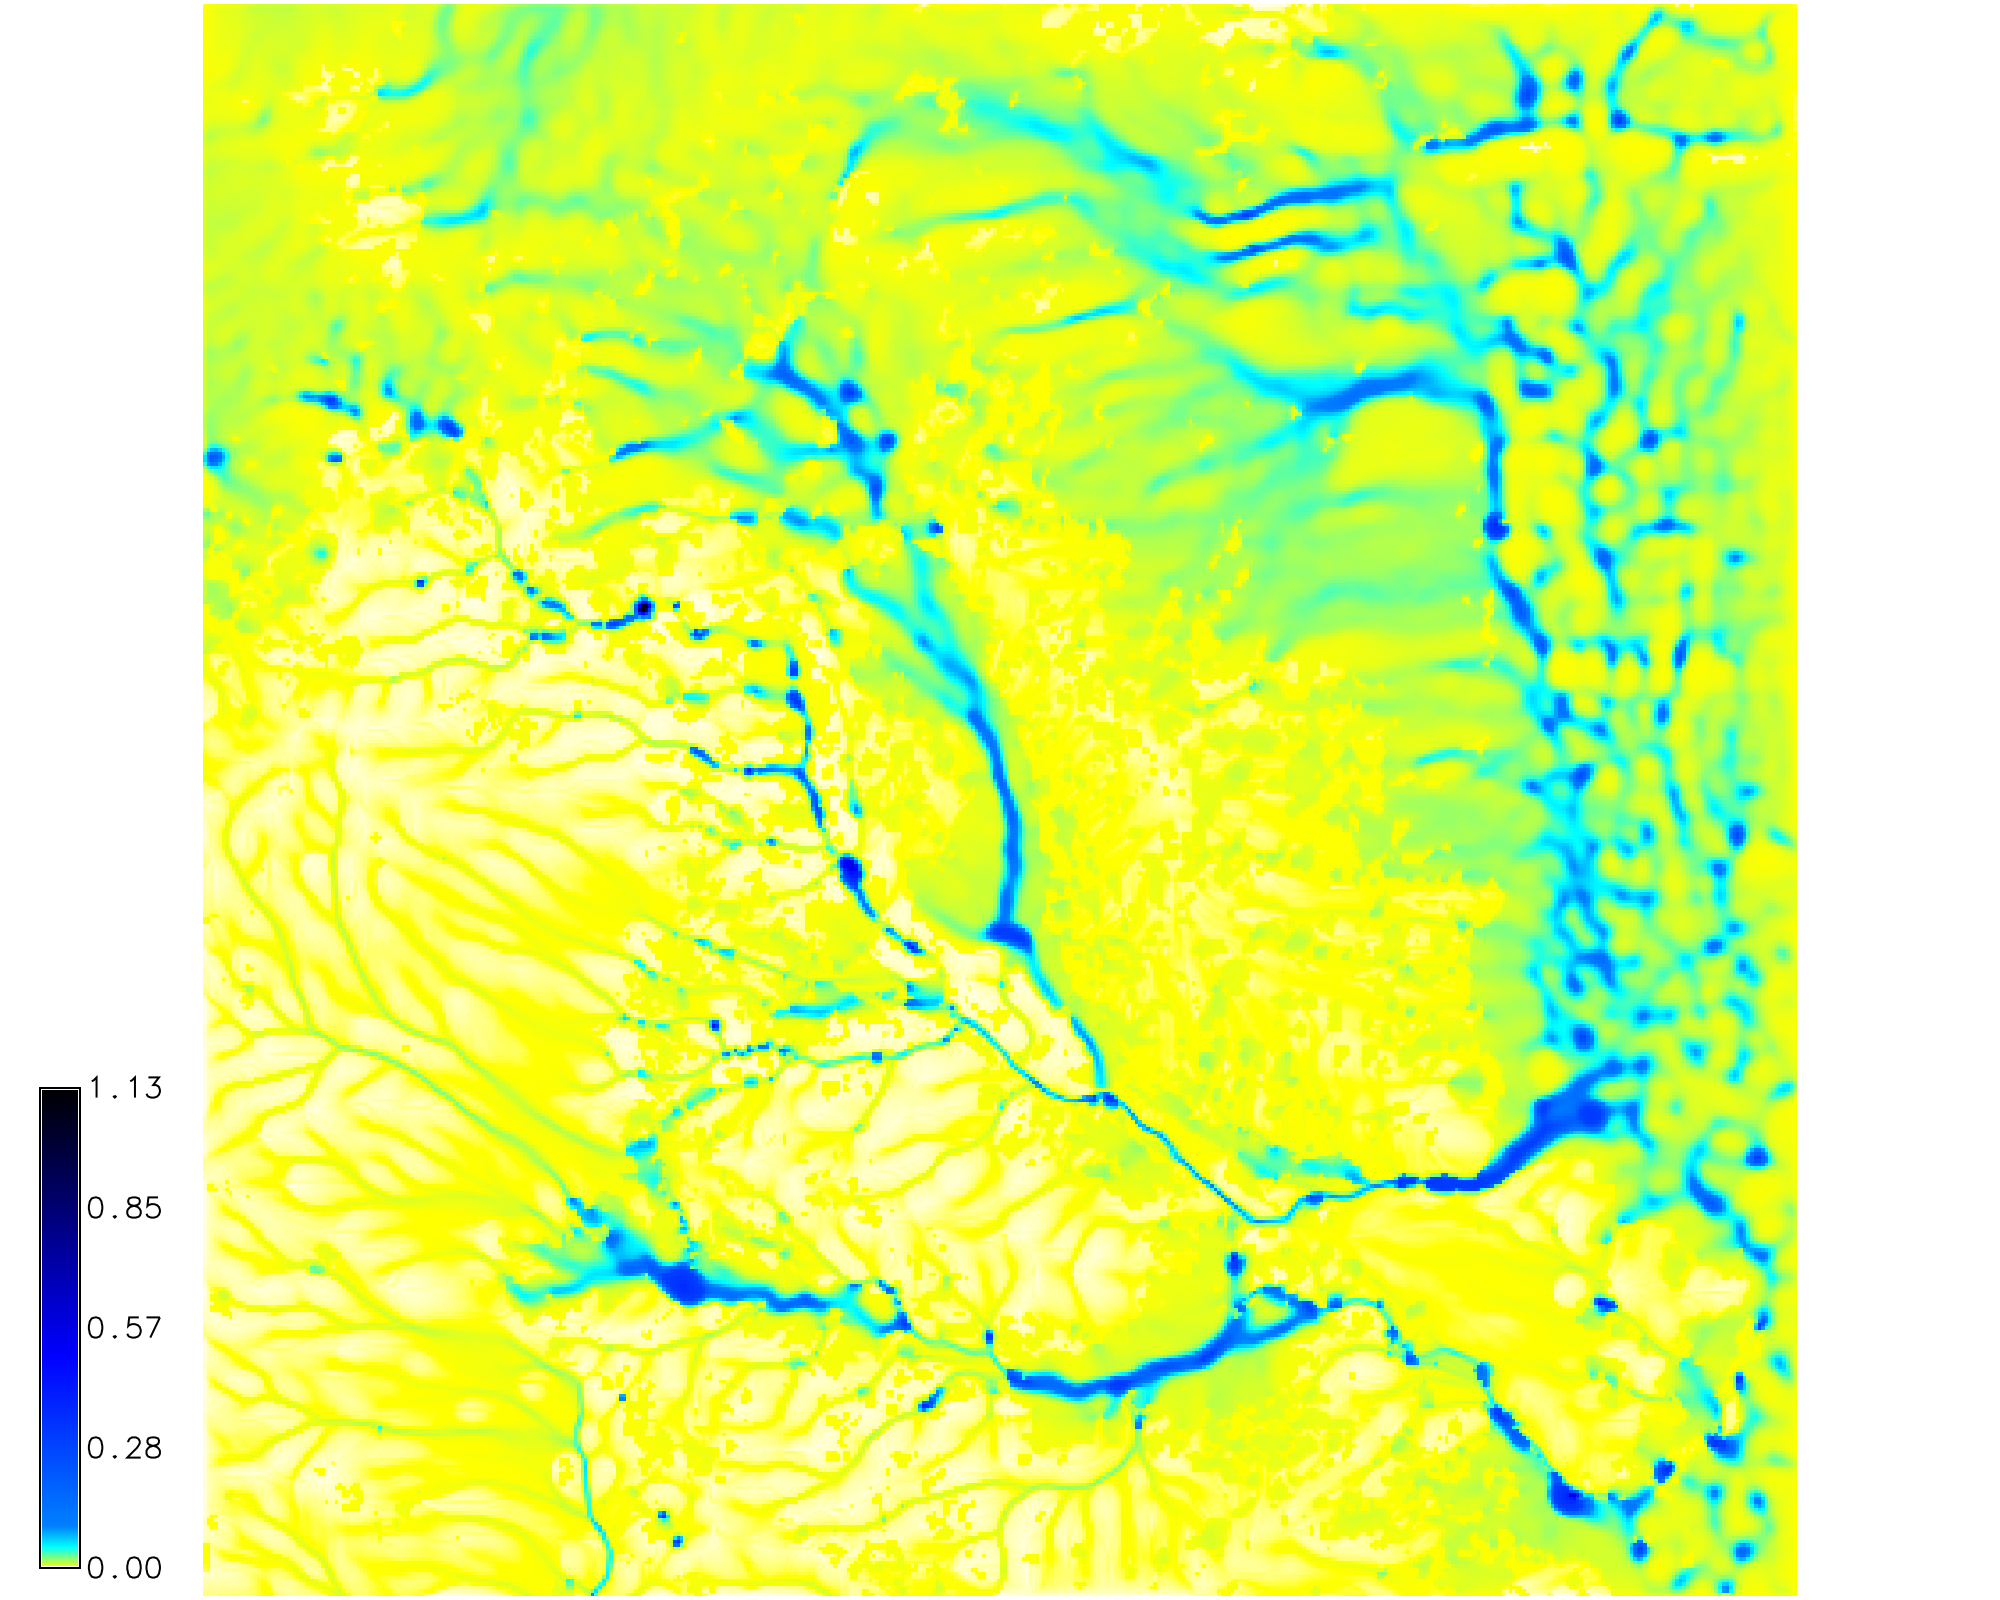
\includegraphics[height=60mm]{../../images/sample_data/depth_2016.png}} &
\multicolumn{1}{c}{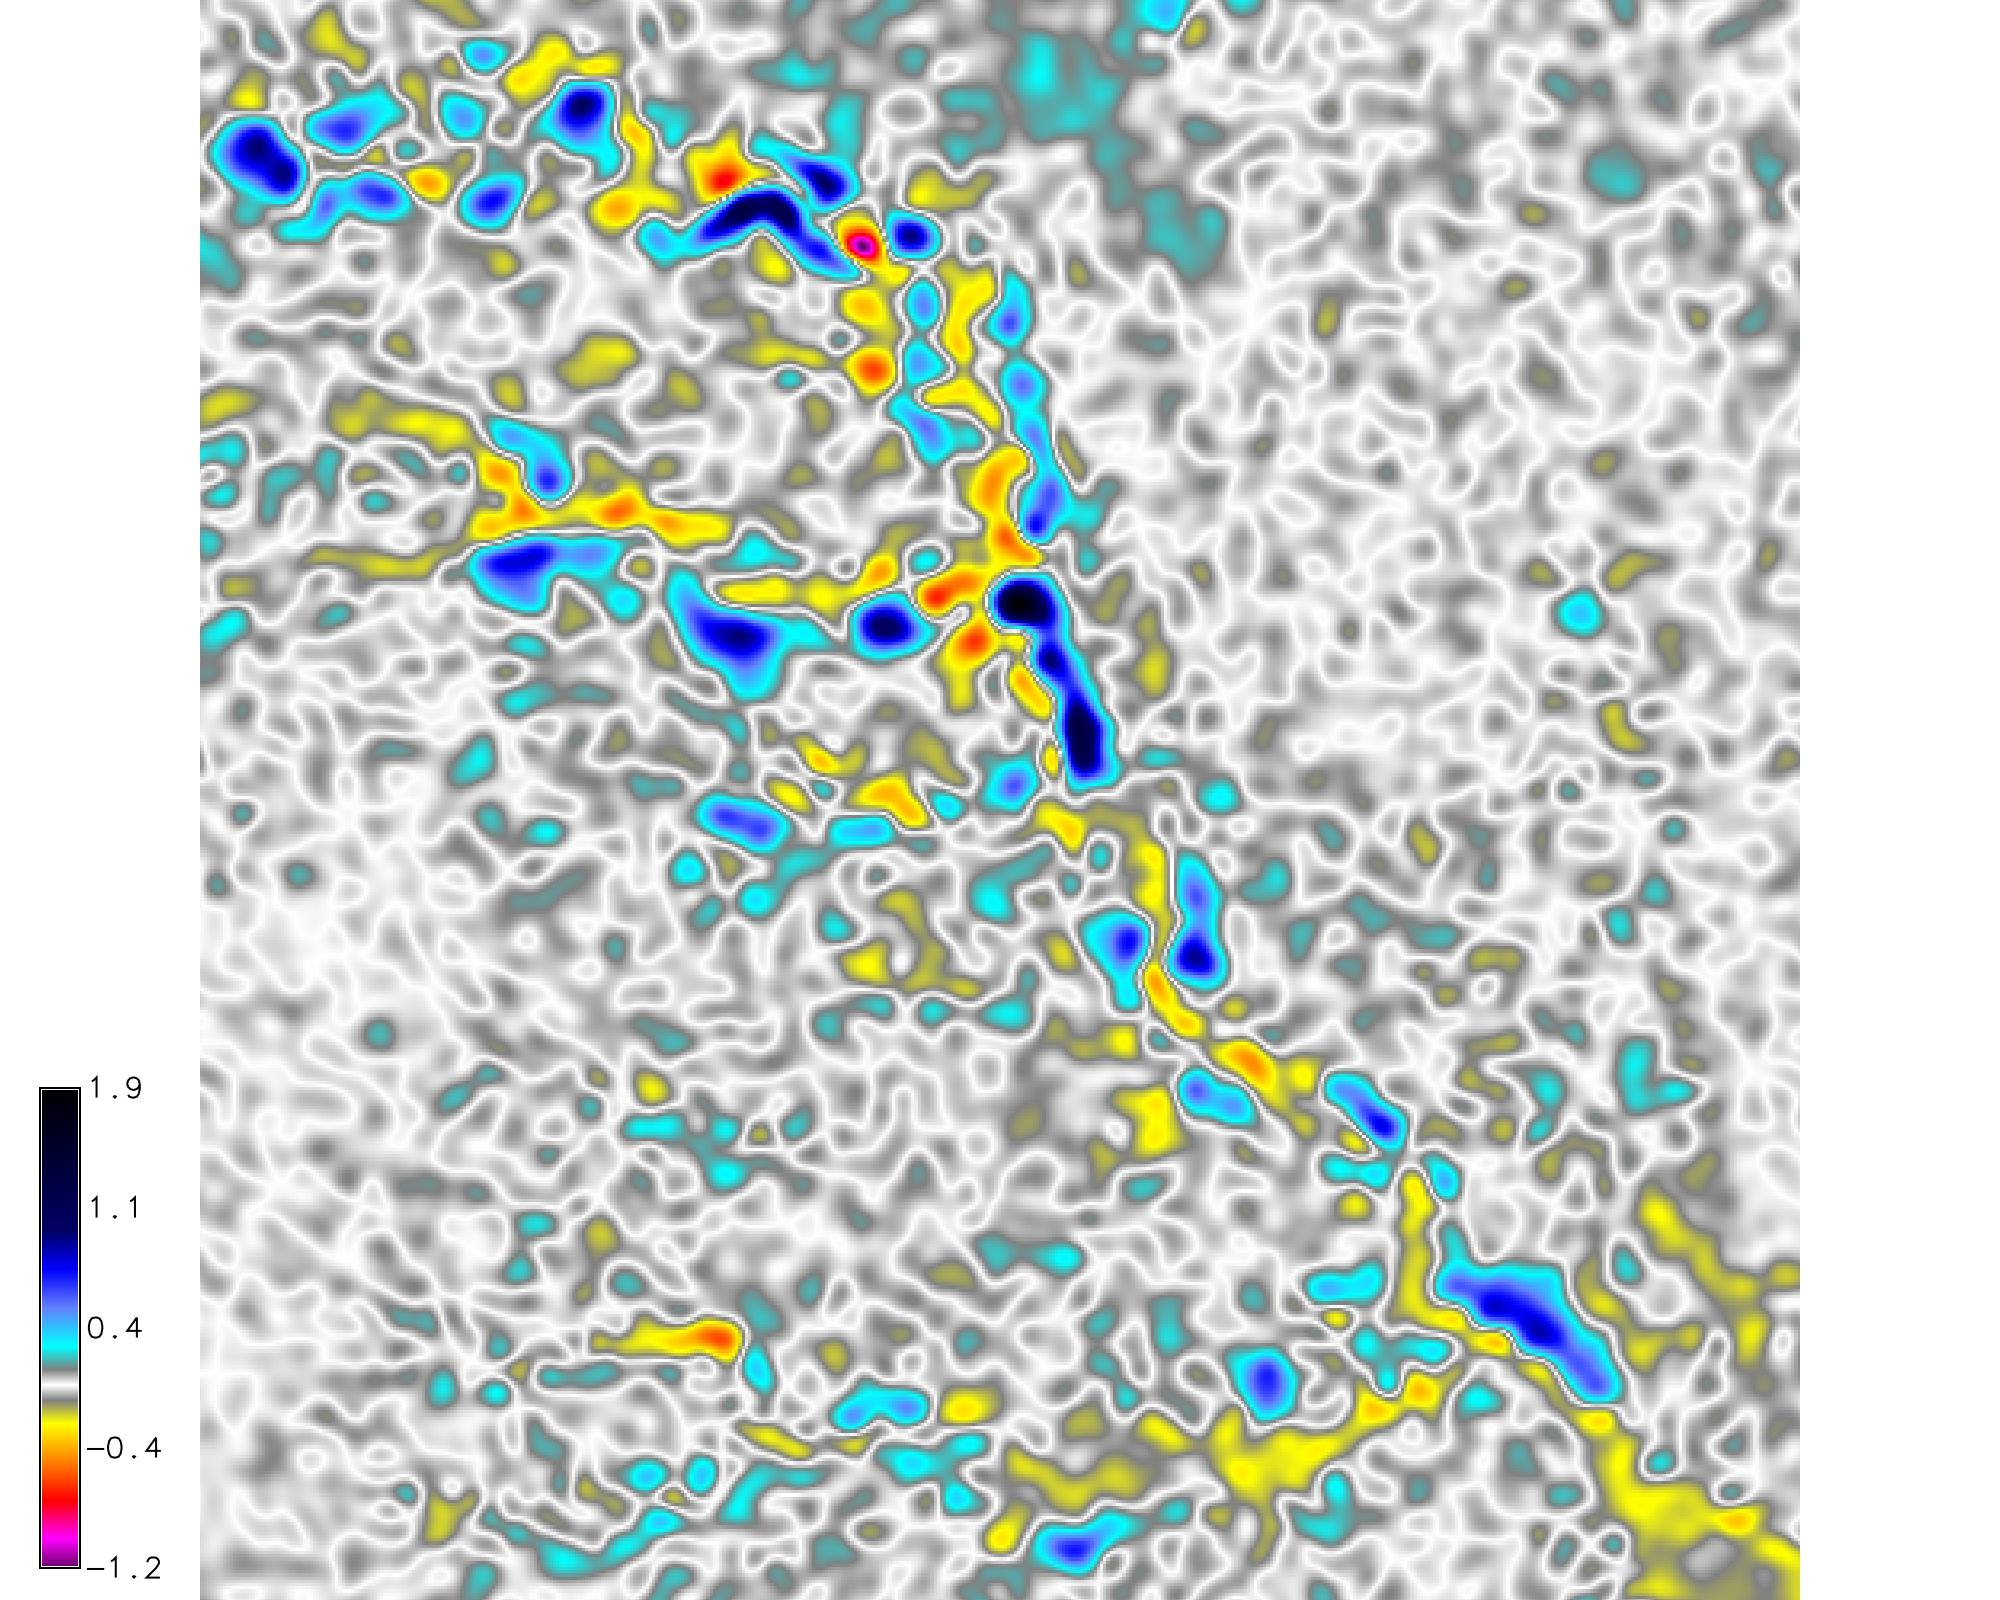
\includegraphics[height=60mm]{../../images/sample_data/gully_difference_2012_2016.png}}\\
\multicolumn{1}{c}{e. Water depth for 10 min event with 50mm/hr} & \multicolumn{1}{c}{f. Difference 2012-2016}\\
%
\end{tabular}
%\caption{Study Landscape, Patterson Branch Creek, Fort Bragg, NC, USA}
%\label{fig:study_area}
%\end{figure}

\end{document}